\documentclass[12pt,letterpaper]{article}
\usepackage[latin1]{inputenc}
\usepackage[spanish]{babel}
\usepackage{amsmath}
\usepackage{amsfonts}
\usepackage{amssymb}
\usepackage{graphicx}
\usepackage[hidelinks]{hyperref}
\usepackage{color}
\graphicspath{{Imagenes/}}
\usepackage[left=2cm,right=2cm,top=2cm,bottom=2cm]{geometry}
\author{M�rquez M�rquez Amairani Ivette}
\title{EV 1.2 OptoAcopladores y Relevadores}
\date{3 de Octubre del 2019}
\begin{document}

\begin{center}
\textbf{\huge{Universidad Politecnica de la Zona \\[0.5cm] Metropolitana de Guadalajara }}
\end{center}

\begin{center}

\includegraphics[width=0.65\textwidth]{UPCDLZMDG5783-logo}\\[2cm]
\end{center}
\vspace{0.1cm}
{\large\textbf{Evidencia:} 1.2 OptoAcopladores y relevadores\\[0.2cm]\textbf{Integrantes:} Bueno Gomez Jorge Heriberto\\[0.2cm]M�rquez M�rquez Amairani Ivette\\[0.2cm]\textbf{Profesor:}Mor�n Garabito Carlos Enrique\\[0.2cm]\textbf{Carrera:} Ing.Mecatronica\\[0.2cm]\textbf{Grupo:} 4�B\\[0.2cm]\textbf{Fecha de entrega:} 4 de Octubre del 2019\\[0.2cm]}\\

\vspace{10cm}
\textbf{1.2 OptoAcopladores y Relevadores}\\[0.3cm]
\textbf{Objetivo:}\\[0.2cm]
Aprender el funcionamiento y estructura de los optocopladores y relevadores en un circuito.\\[0.5cm]
\vspace{0.2cm}
\textbf{Materiales:}
\begin{itemize}
\item Relevadores
\item Optoacopladores
\item Resistencias
\item Transistores
\item LED�S
\item Arduino
\item Fuente de poder
\item Protoboard
\end{itemize}
\vspace{0.2cm}
\textbf{Procedimiento:}
\begin{enumerate}
\item Primero se analizo el siguiente circuito para realizar los c�lculos que se necesitan antes de armar el circuito.\
\begin{figure}[h]
\begin{center}
\centering
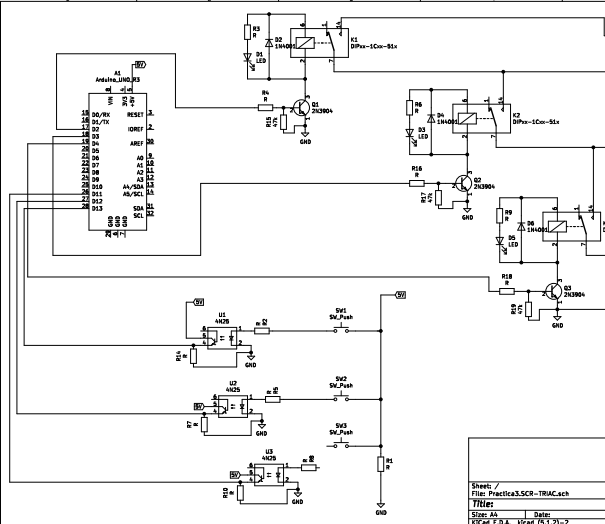
\includegraphics[width=0.50\textwidth]{Imagenes/Captura_1.PNG} 
\caption{Diagrama del circuito en el programa ORCAD}
\end{center}
\end{figure}
\vspace{10cm}
\item Calculamos\
\begin{itemize}
\item OptoAcoplador\\
$$Vf=1.15v$$
$$If=10mA$$
\item Transistor\\
$$R=\dfrac{(5v-0.6)250}{12mA}$$
$$R=1.528 \Omega$$
\item LED\\
$$LED=\dfrac{(12v-1.15v)}{10mA}$$
$$LED=1.085 \Omega$$
\end{itemize}
\item Por ultimo se realiza el circuito con los materiales vistos anteriormente a base del circuto y de los calculos.
\end{enumerate}
\textbf{\large{Bibliograf�as}}\
\begin{center}
\emph{Creative Commons BY NC SA. (2013). INEVITABLE.eu. Obtenido de La electronica simple y clara.} Obtenido de: \textcolor{blue}{ https://www.inventable.eu/controlar-rele-con-transistor/}\\[0.3cm]
\end{center}
\end{document}